\documentclass{article}

% if you need to pass options to natbib, use, e.g.:
\PassOptionsToPackage{numbers, compress}{natbib}
% before loading nips_2017
%
% to avoid loading the natbib package, add option nonatbib:
% \usepackage[nonatbib]{nips_2017}

\usepackage[final]{nips_2017}


%\usepackage[square,numbers]{natbib}
\bibliographystyle{abbrvnat}


\usepackage[utf8]{inputenc} % allow utf-8 input
\usepackage[T1]{fontenc}    % use 8-bit T1 fonts
\usepackage{hyperref}       % hyperlinks
\usepackage{url}            % simple URL typesetting
\usepackage{booktabs}       % professional-quality tables
\usepackage{amsfonts}       % blackboard math symbols
\usepackage{nicefrac}       % compact symbols for 1/2, etc.
\usepackage{microtype}      % microtypography
\usepackage{subcaption}
\usepackage{graphicx}

% Choose a title for your submission
\title{Story Cloze Test}


\author{Lea Fritschi \qquad Beat Hubmann \qquad  Maya V\"ogeli \qquad   Lukas Wampfler}

\begin{document}
% \nipsfinalcopy is no longer used

\maketitle

% We do not require you to write an abstract. Still, if you feel like it, please do so.
%\begin{abstract}
%\end{abstract}

\section{Introduction}
The given task was to design and implement an attempt at the 'Story Cloze Test' \cite{DBLP:journals/corr/MostafazadehCHP16}, a framework for evaluating story understanding and script learning.
After some disappointing initial attempts with an attention-augmented encoder-decoder model, we decided to apply the idea to learn sentence vector representations to predict the context of a sentence \cite{eff_framework} to the 'Story Cloze Test'.


\section{Methodology}

In our implementation, we follow the approach of {\bf quick thoughts}, as proposed in \cite{eff_framework}. Unlike the approach of generating a target sequence from an input sentence commonly used for this class of problems, our chosen approach attempts to choose the correct target sentence of an input sentence from a set of given candidate sentences based on learned sentence encodings. A massive benefit of this approach is that it allows for a large (i.e. rich) vocabulary size as no target sequence needs to be generated from the encoded input and thus there is no efficiency and numerical stability bottleneck at that point. Also, this approach uses the very simple and efficient classifier $c(u, v) = u^\top v$ to force the encoders to learn relevant sentence representations. Finally, the approach not only allows for but actually relies on large minibatch sizes and thus can be trained efficiently.

\section{Model}



Our model follows closely what has been described in \cite{eff_framework}. Therefore, our model description is taken and adapted from \cite{eff_framework}: \\[.1cm]
Let $f$ and $g$ be two parametrized functions that each take a sentence as input and encode it into a fixed length vector. Let $s$ be a given sentence. Let $S_{ctxt}$ be the set of sentences appearing in the context of $s$ in the training data (in our case: for the second to fourth sentence of a story, the context consists of two sentences: the one sentence before and the one after. For the first and last sentence of each story however, the context consists of one sentence only: the second resp. the fourth one) Let $S_{cand}$ be the set of candidate sentences considered for a given context sentence $s_{ctxt} \in S_{ctxt}$. In other words, $S_{cand}$ contains a valid context sentence $s_{ctxt}$ (ground truth) and many other non-context sentences (in our case, we used the minibatch of $100$ sentences as $S_{cand}$), and is used for the classification objective. \\[.2cm]
For a given sentence position in the context of $s$, the probability that a candidate sentence \\$s_{cand}\in S_{cand}$ is the correct sentence (i.e. really appearing in the context of $s$) for that position is given by
$$
p(s_{cand} \, | s, S_{cand}) = \frac{\exp(c(f(s), g(s_{cand})))}{\sum_{s'\in S_{cand}}\exp(c(f(s), g(s')))}
$$
where $c$ is  a scoring function/classifier. We use $c(u, v) = u^\top v$ as  a classifier. \\[.3cm]
The training objective maximizes the probability of identifying the correct context sentences for each sentence in the training data $D$.
$$
\sum_{s\in D} \sum_{s_{ctxt} \in S_{ctxt}} \log \, p(s_{ctxt} \, | s, S_{cand})
$$

For the encoding functions $f$ and $g$, we settled on bidirectional RNNs with 600 GRU cells each. \\[.1cm]
When evaluating the trained model, the fourth story sentence is fed to the encoder $f$ and the classifier then decides which of the two candidate endings encoded by encoder $g$ is more probable (see figure).
\begin{figure}[h]
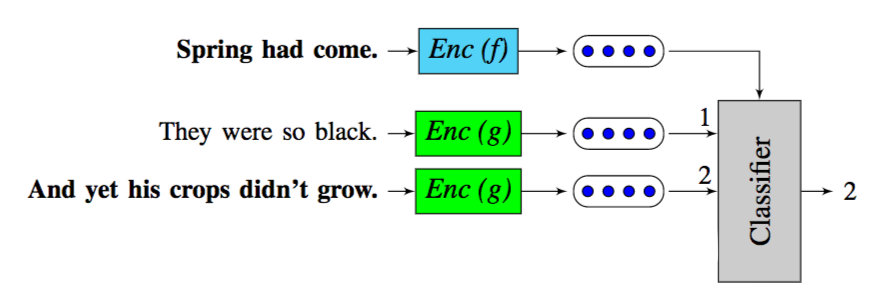
\includegraphics[width=0.8\textwidth]{fig_architecture_test}


\caption{During validation, we use a classifier to decide which of the candidate sentences is the correct ending of the story; figure taken from \cite{eff_framework} and adapted}
\end{figure}

\section{Training}
For trainable word embeddings, we based on with GloVe pre-trained word embeddings in $300$ dimensions \cite{pennington2014glove}. 
As training data, we exclusively used the given corpus of $88161$ five sentence stories. In these stories, there were no alternative (wrong) ending sentences. 
A context scope of +/- 1  was used, where the previous and the next sentences are predicted given an input sentence.
After measuring accuracy on the validation set, we chose hyperparameters to be a minibatch size of $100$ sentences (i.e. $20$ cloze stories with $5$ sentences each) with a dropout rate of $0.25$. We trained over $5$ epochs to minimize cross-entropy with Adam Optimizer at a learning rate of $1e-3$.
Due to the efficient nature of this approach, total training time on a single GTX 1080 Ti GPU was well under an hour.


\section{Experiments}
On the given validation set, we achieve an accuracy of $0.612$ using the parameters mentioned above. The trained model then achieves an accuracy of 0.618 on the assigned test set. This result is comparable with respect to what has been published earlier \cite{mostafazadeh-EtAl:2016:N16-1, Roemmele2017AnRB}.

\section{Conclusion}
Due to the limited scope and time of this project, we felt we couldn't fully exploit the benefits of our chosen approach. For further investigation, the use of more sophisticated embeddings (case sensitive; Skip-thoughts) as well as using more sophisticated RNN encoding functions would look promising.

%\bibliographystyle{plain}
\bibliography{bibliography} 
\end{document}
